\documentclass[11pt]{article}
\usepackage[margin=0.72in]{geometry}
\usepackage{amsmath,amssymb,bm,booktabs,graphicx,float}
\usepackage[colorlinks=true,linkcolor=blue!55!black]{hyperref}
\usepackage{xcolor}
\IfFileExists{placeins.sty}{\usepackage{placeins}}{\newcommand{\FloatBarrier}{\clearpage}}
\graphicspath{{V2_figure/realdata/}}
\newcommand{\Normal}{\mathcal N}
\newcommand{\E}{\mathbb E}
\newcommand{\Var}{\operatorname{Var}}
\newcommand{\EPSS}{\operatorname{EPSS}}
\newcommand{\IG}{\operatorname{IG}}
\newcommand{\logit}{\operatorname{logit}}
\setlength{\tabcolsep}{5pt}
\renewcommand{\arraystretch}{1.12}
\title{Prior Impact: Three Case Studies}
\author{Fangzhou Cao}
\date{}

\begin{document}
\maketitle

Each comparison reports Reimherr, Wiesenfarth, Jones, and CP, in that order.
R/W use mean risk for the normal and Eight Schools cases, and median risk
for lupus. Here median refers to aggregation of the internal pseudo-data
losses before matching, not to a posterior median or a median across datasets.
Simulation surfaces report the arithmetic mean of dataset-specific EPSSs. CP uses deletion and the loss
\[
 H_1=(c_1-c_2)^2+\{\min(c_1,c_2)-0.95\}^2,
 \qquad c_1=P(R_Q),\quad c_2=Q(R_P),
\]
where $R_P,R_Q$ are the respective 95\% posterior regions. Matching is
performed within each path before averaging signed selections.

\section{Normal sampling with unknown mean and variance}

\subsection{Simulation}
For each of $R=50$ datasets,
\[
 X_i\mid\mu,\sigma^2\overset{\mathrm{iid}}\sim\Normal(\mu,\sigma^2),
 \qquad n=20,\qquad(\mu^{\mathrm{true}},\sigma^{2,\mathrm{true}})=(0,1).
\]
The informative and baseline priors are
\[
 \pi:\quad \mu\mid\sigma^2\sim\Normal(\mu_0,0.2\sigma^2),
 \quad\sigma^2\sim\IG(\kappa,\eta),
 \qquad b(\mu,\sigma^2)\propto(\sigma^2)^{-1},
\]
with $\IG(\kappa,\eta)$ density proportional to
$(\sigma^2)^{-\kappa-1}\exp(-\eta/\sigma^2)$. Write
$a=\E_\pi(\sigma^2)$ and $v=\Var_\pi(\sigma^2)$; then
\[
 \kappa=2+a^2/v,\qquad \eta=a(\kappa-1).
\]
The $17\times15$ prior grid is
\begin{align*}
 \mu_0&\in\{-4,-3.5,\ldots,4\},\\
 a&\in\{0.25,0.35,0.5,0.7,0.85,1,1.15,1.3,1.5,1.75,2,2.5,3,4,5\}.
\end{align*}
We display $v=20$. The five posterior targets, in figure-row
order, are
\[
 (\mu,\log\sigma^2),\quad(\mu,\sigma^2),\quad
 \mu,\quad\log\sigma^2,\quad\sigma^2.
\]
One EPSS unit is one normal observation. R/W average $B=1000$ internal
losses; Jones and CP average 500 pathwise selections. Reimherr uses
bootstrap posterior MSE. Wiesenfarth uses plug-in likelihood pseudo-data and squared posterior-mean error.

% \begin{figure}[p]
% \centering
% 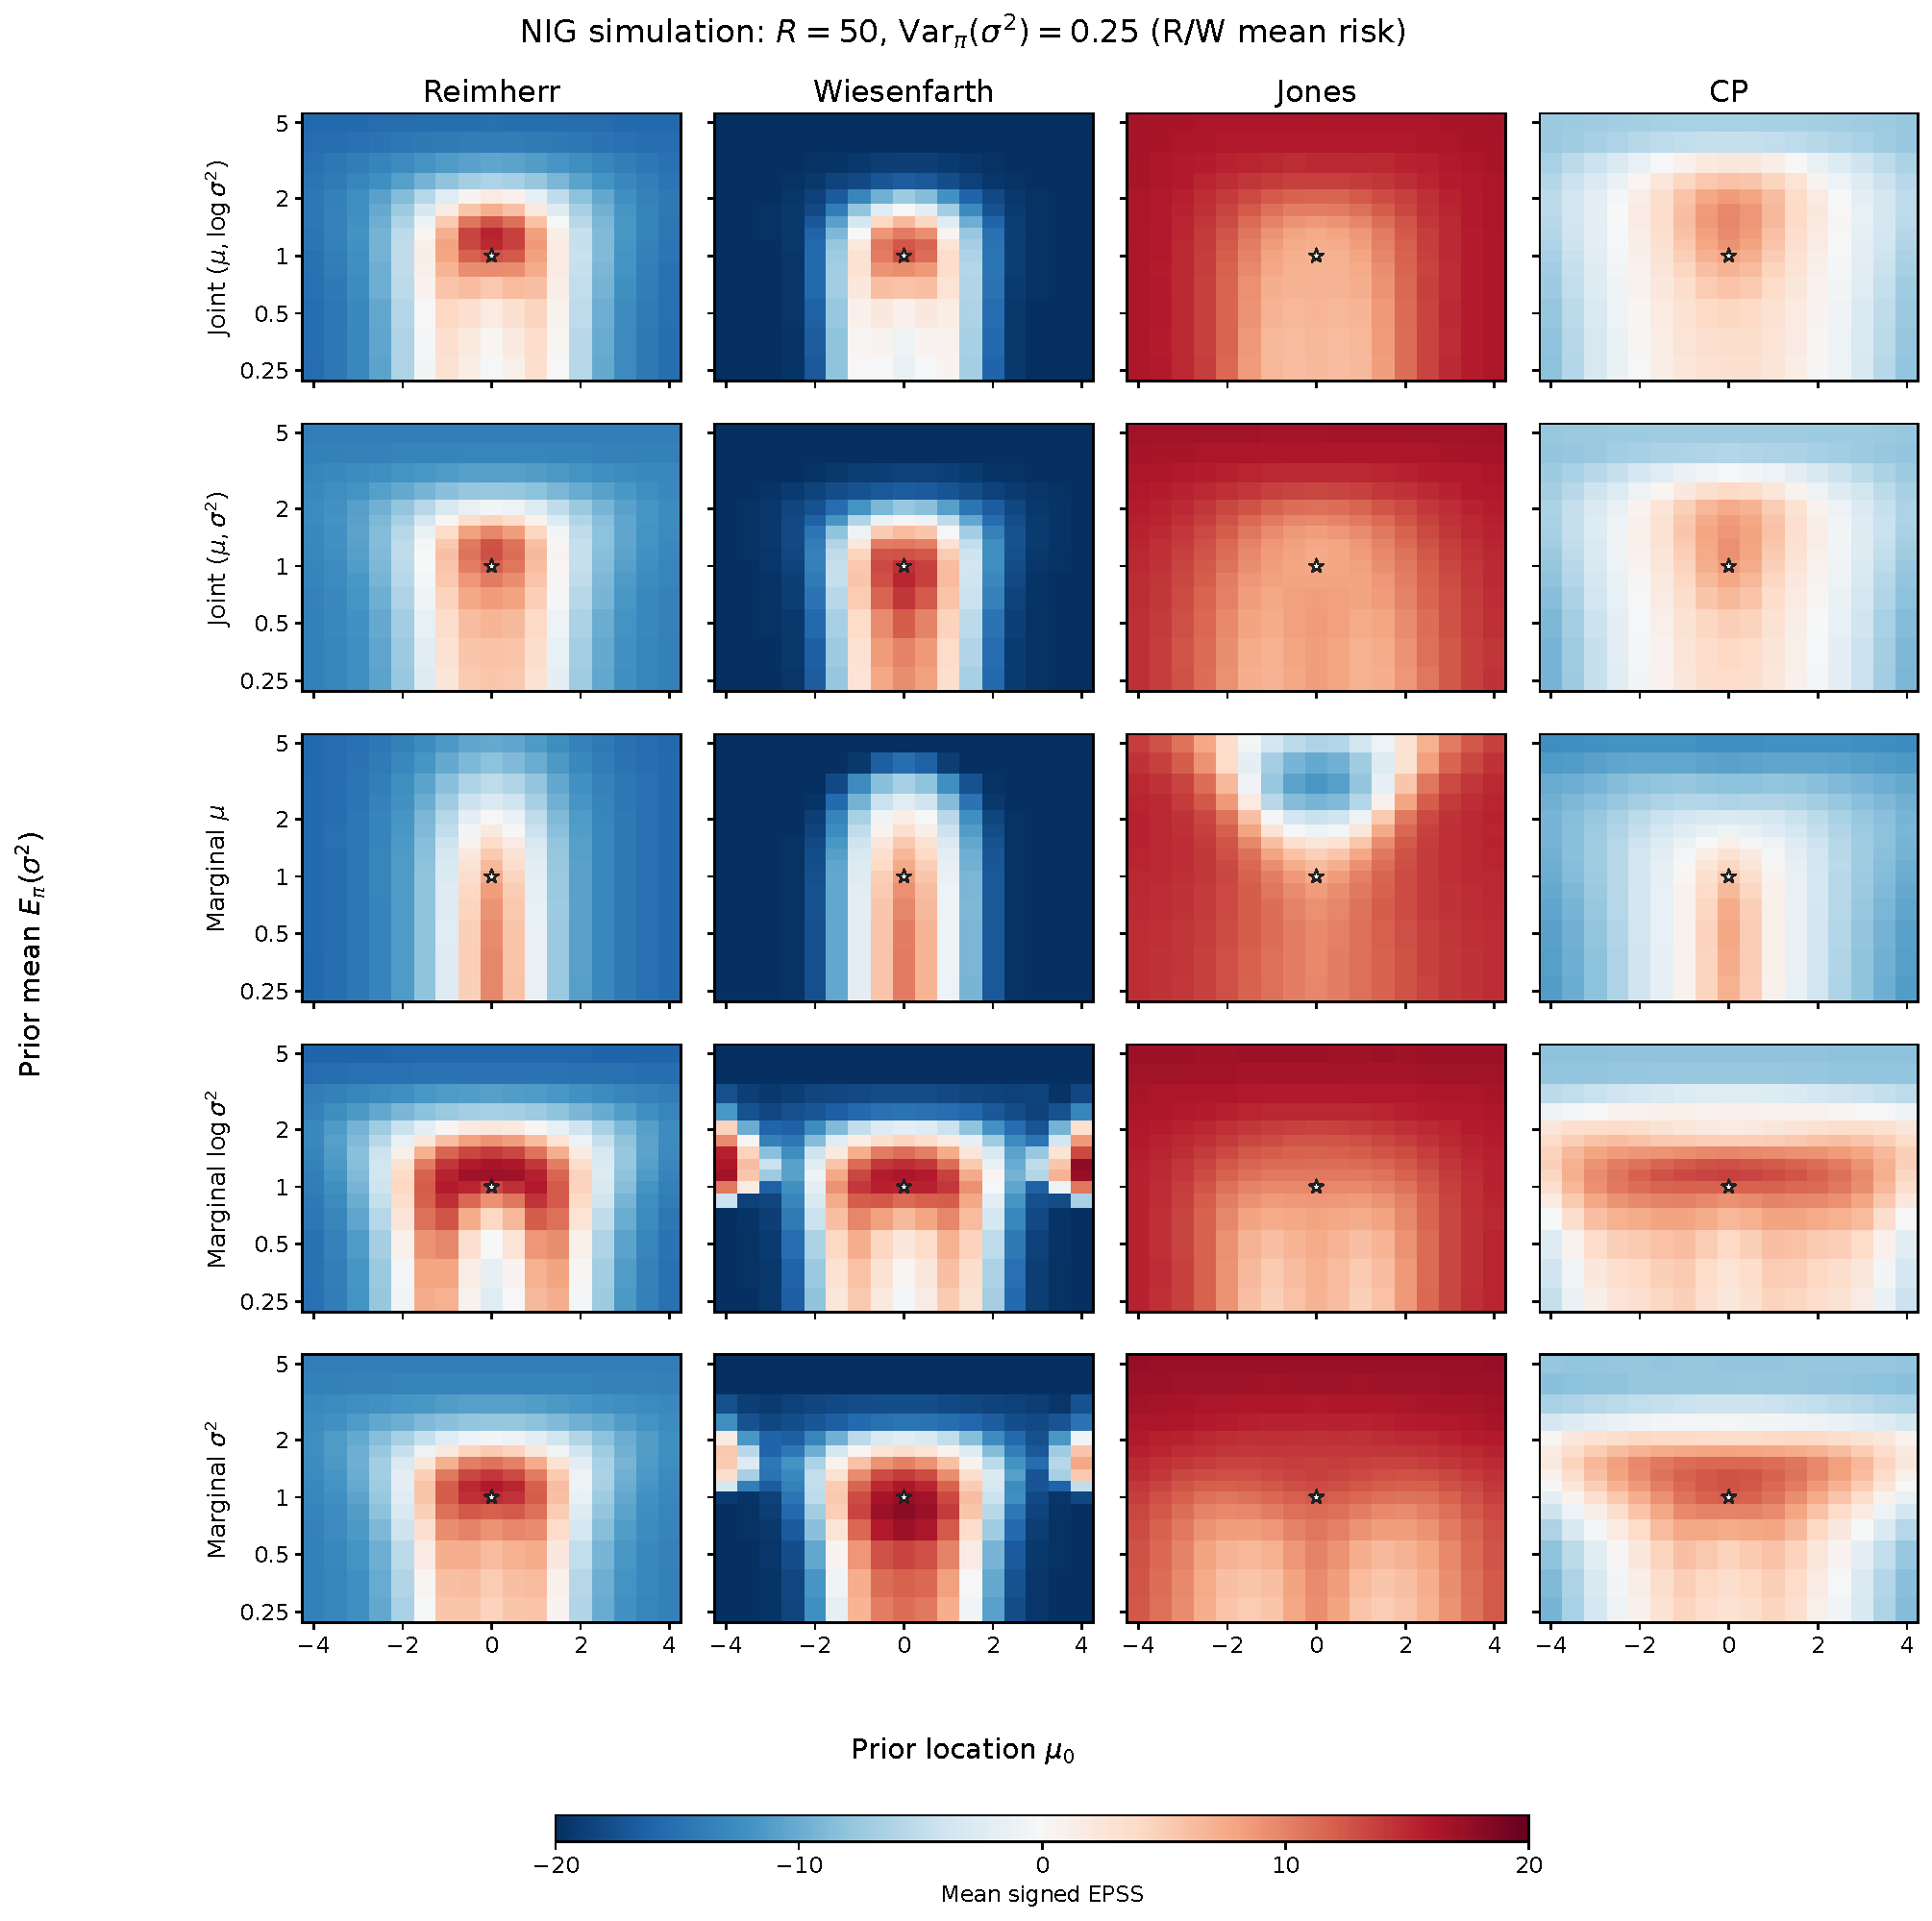
\includegraphics[width=\linewidth,height=.81\textheight,keepaspectratio]{NIG/simulation_var_0p25_5x4.pdf}
% \caption{Normal simulation, $v=0.25$: mean EPSS over 50 datasets.
% Rows are the five stated posterior targets; columns are Reimherr,
% Wiesenfarth, Jones, and CP. The star marks $(\mu_0,a)=(0,1)$.
% The prior-variance mean axis is logarithmic; all panels use the common
% signed EPSS scale $[-20,20]$. R/W use mean risk.}
% \end{figure}
\begin{figure}[p]
\centering
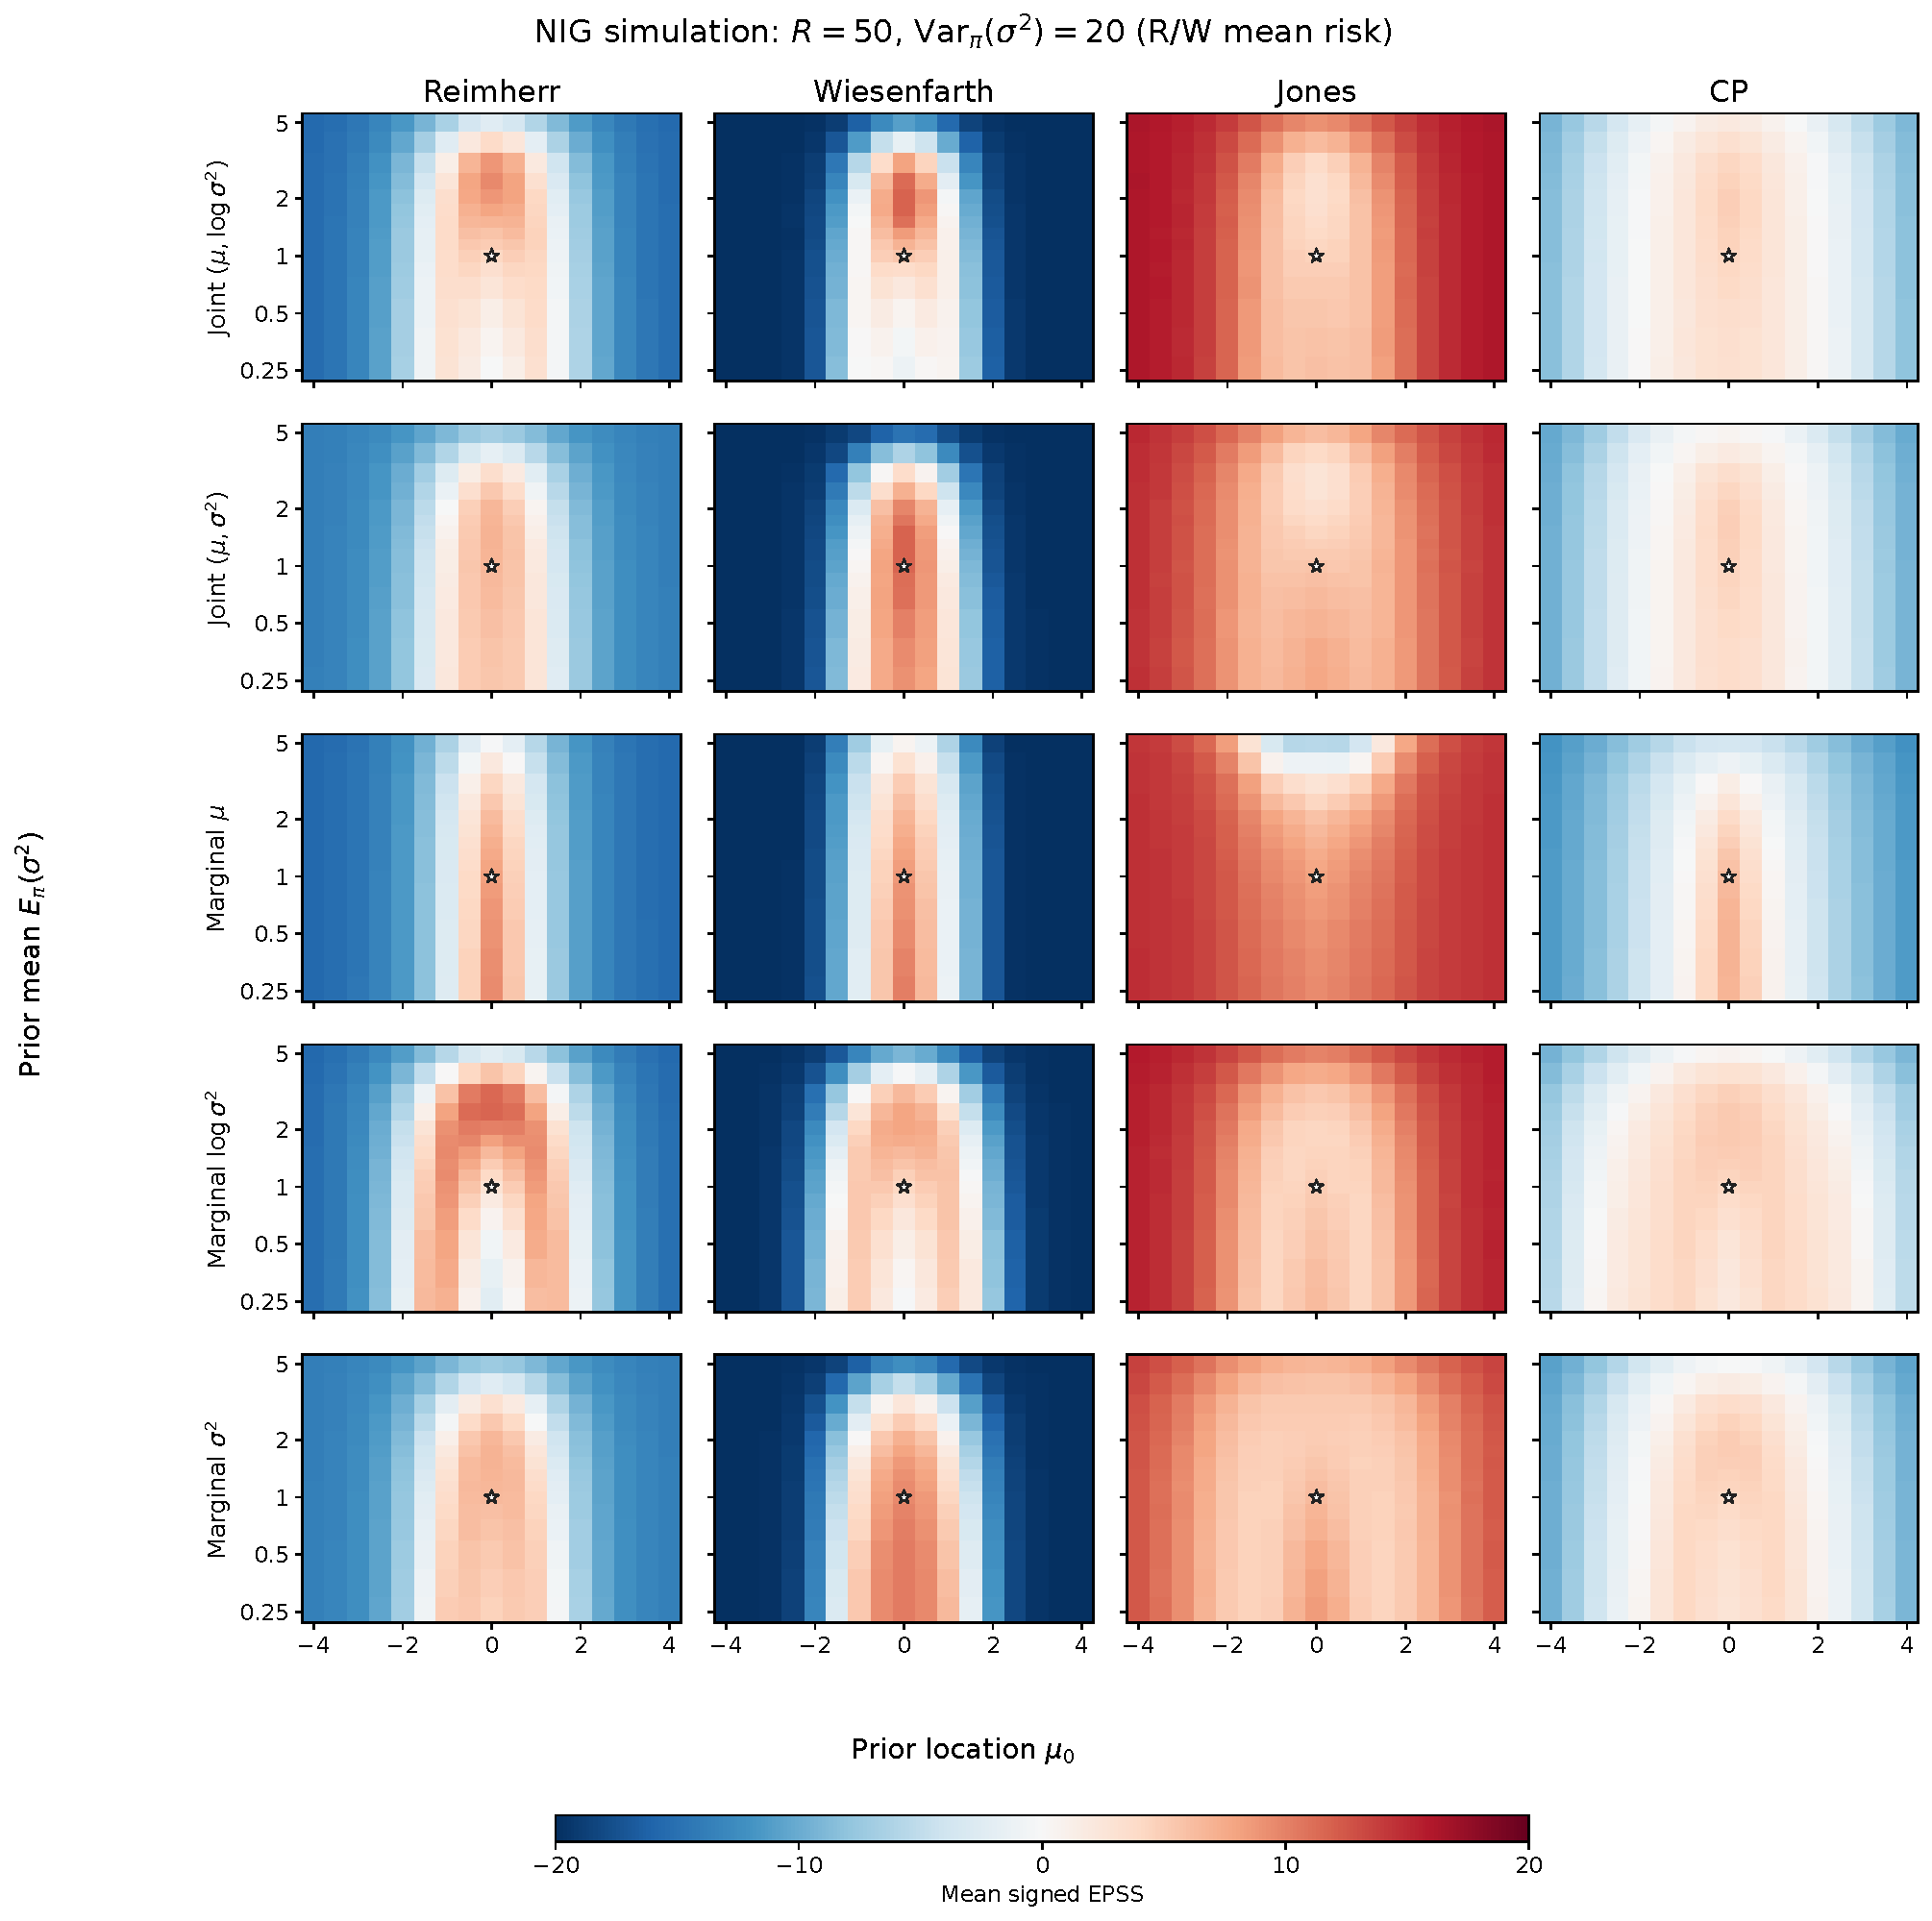
\includegraphics[width=\linewidth,height=.81\textheight,keepaspectratio]{NIG/simulation_var_20_5x4.pdf}
\caption{Normal simulation, $v=20$: mean EPSS over 50 datasets.
Rows are the five stated posterior targets; columns are Reimherr,
Wiesenfarth, Jones, and CP. The star marks $(\mu_0,a)=(0,1)$.
The prior-variance mean axis is logarithmic; all panels use the common
signed EPSS scale $[-20,20]$. R/W use mean risk.}
\end{figure}
\FloatBarrier

\subsection{Real data: midge wing lengths}
The nine wing lengths (mm) used in Hoff's normal-model example are
\[
 y=(1.64,1.70,1.72,1.74,1.82,1.82,1.82,1.90,2.08),
 \qquad \bar y=1.80444.
\]
The likelihood and Jeffreys baseline are as above, but the informative
prior is
\[
 \mu\mid\sigma^2\sim\Normal(\mu_0,\sigma^2),
 \qquad\sigma^2\sim\IG(0.5,0.005).
\]
Only $\mu_0$ varies. Its 82-point grid is
\[
 \{1.30,1.32,\ldots,1.78\}\cup
 \{1.800,1.805,\ldots,2.000\}\cup
 \{2.02,2.04,\ldots,2.30\}\cup\{\bar y\}.
\]
Hoff's original location is $\mu_0=1.9$. The targets are
$\mu/0.1$, $\log(\sigma^2/0.01)$, and their joint posterior. R/W use
$B=1000$ mean-risk pseudo-datasets and signed grids $-3{:}40$ and
$-40{:}5$, respectively. Jones uses $0{:}40$ additions and CP $0{:}5$
deletions, each with 500 paths.

\begin{figure}[p]
\centering
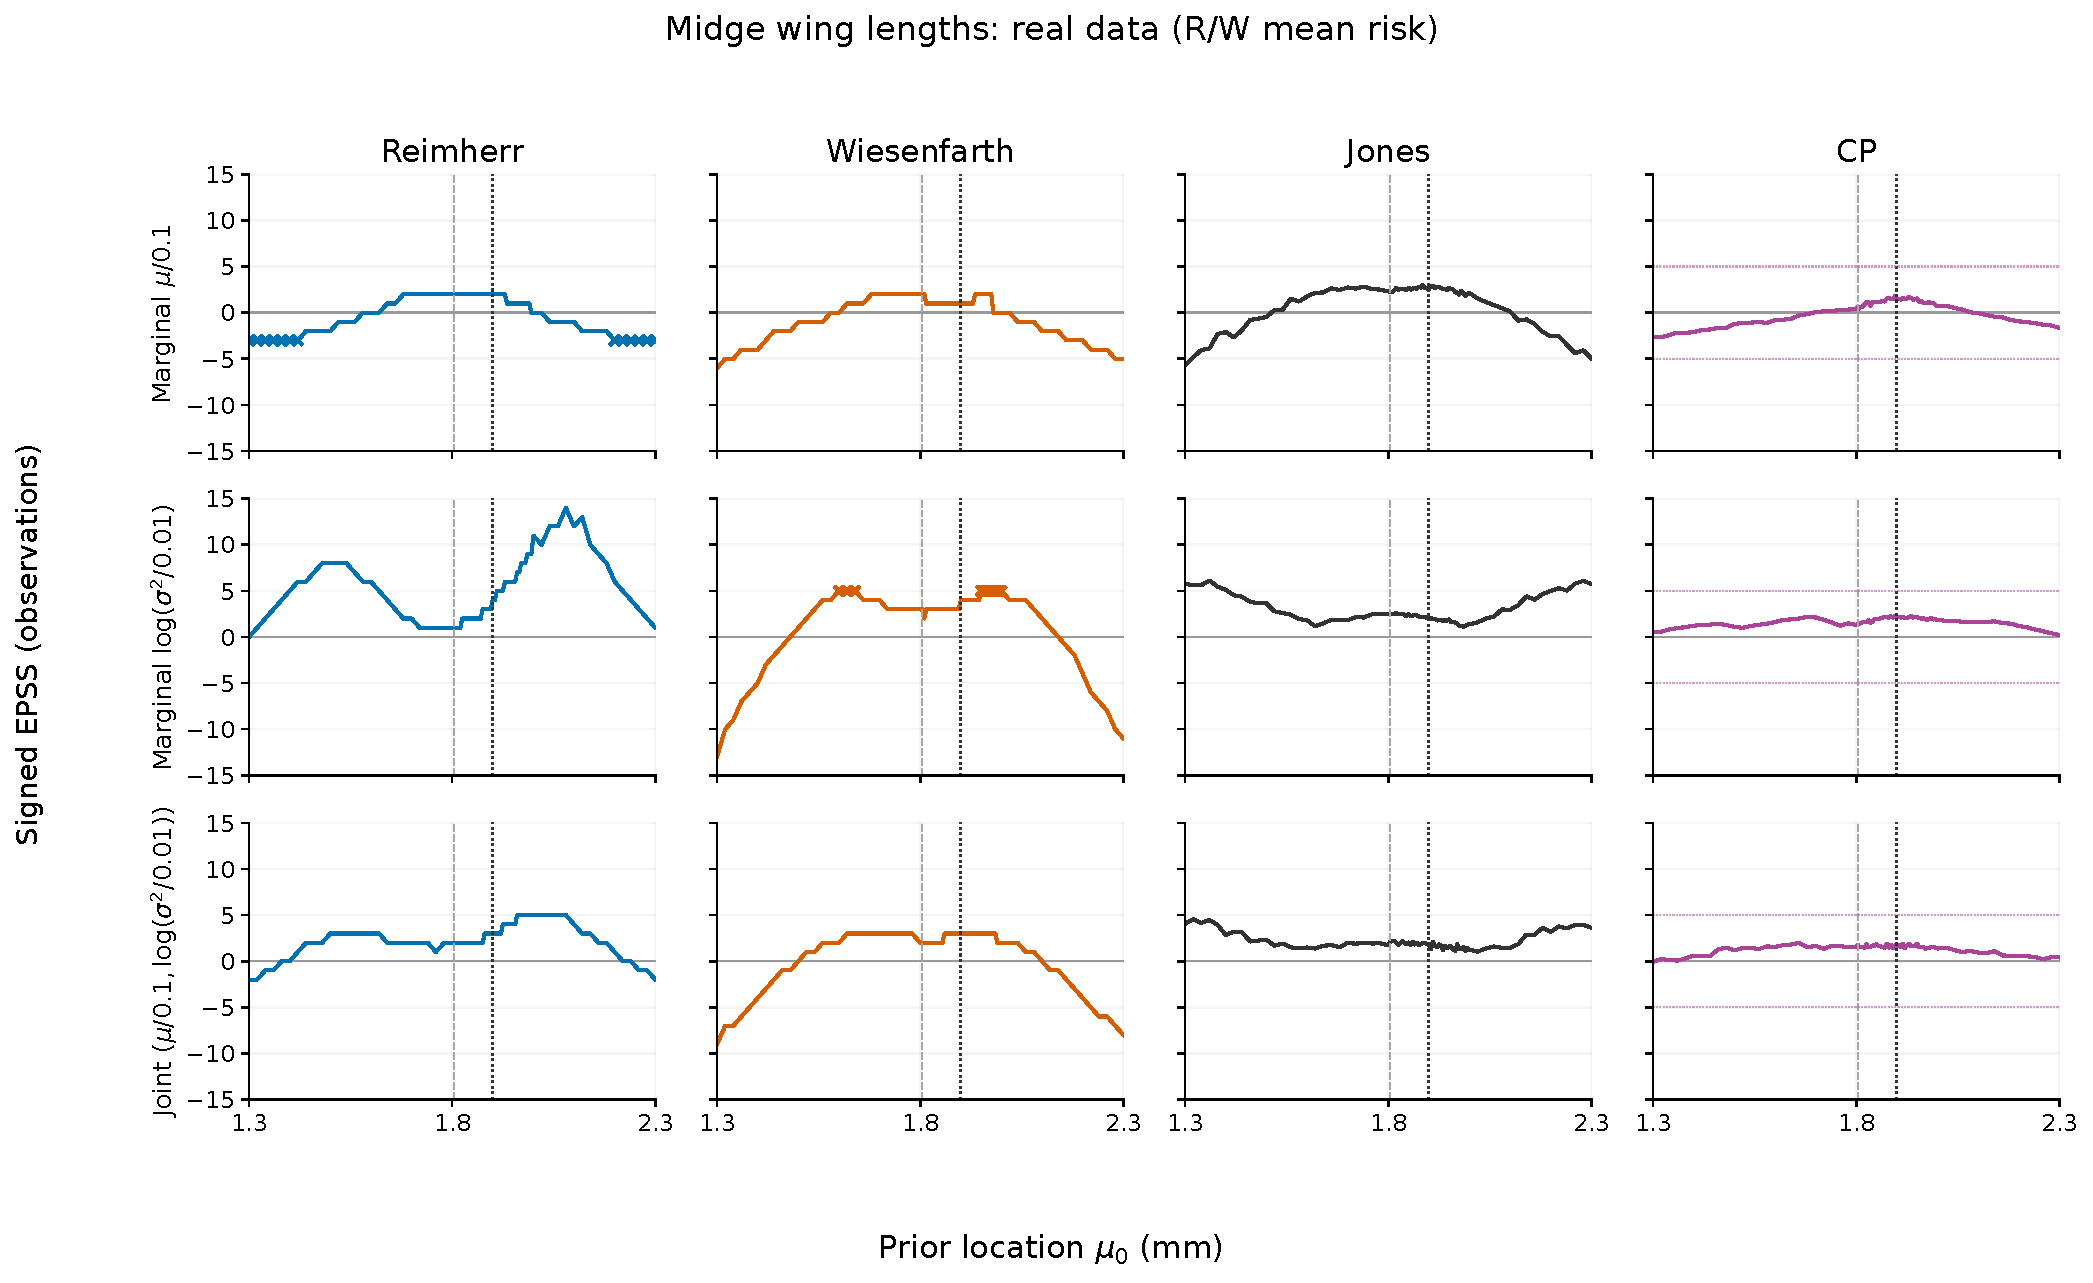
\includegraphics[width=\linewidth,height=.78\textheight,keepaspectratio]{NIG/real_3x4.pdf}
\caption{Midge wing lengths: one observed dataset, with R/W mean risk.
Gray dashed and black dotted vertical lines mark the observed mean and
original prior location 1.9, respectively; neither is a known truth.
Crosses mark R/W endpoint selections; purple dotted lines mark CP limits
$\pm5$. All panels retain the original common EPSS axis $[-15,15]$.
No between-dataset uncertainty band applies.}
\end{figure}
\FloatBarrier

\section{Lupus logistic regression}

\subsection{Data, likelihood, and priors}
The 55 patient records, including 18 positive responses, are reconstructed
from the grouped counts
\[
\begin{array}{c|rrrrr}
 x&0&0.5&1&1.5&2\\\hline
 y=0&31&2&2&0&2\\
 y=1&5&0&2&6&5
\end{array}
\]
and modeled as
\[
 x_i^\star=\frac{x_i-\bar x}{2s_x},\qquad
 Y_i\mid\beta\sim\operatorname{Bernoulli}(p_i),\qquad
 \logit(p_i)=\beta_0+\beta_1x_i^\star,
\]
where $\bar x=0.5090909$, $2s_x=1.5334651$, and $s_x$ is the
sample standard deviation of the 55 raw predictors. For a raw dose $x$,
$p(x)=\logit^{-1}\{\beta_0+\beta_1(x-\bar x)/(2s_x)\}$.
The independent coefficient priors are
\begin{align*}
 \pi:\quad&\beta_0\sim t_7(\mu_{\beta_0},10),
             &\beta_1&\sim t_7(\mu_{\beta_1},2.5),\\
 b:\quad&\beta_0\sim t_7(0,10),
             &\beta_1&\sim t_7(0,1000),
\end{align*}
where the second argument denotes scale. Both experiments use the 561-cell grid
\[
 \mu_{\beta_0}\in\{-5,-4.5,\ldots,3\},\qquad
 \mu_{\beta_1}\in\{-5,-4.5,\ldots,11\}.
\]
One EPSS unit is one patient-level predictor--response pair.

For target $T$, set $z_b=\E_b[T(\beta)\mid y]$. R/W use the losses
\[
 L_R(D)=\operatorname{tr}\{\operatorname{Cov}(T\mid D)\}
       +\|\E(T\mid D)-z_b\|^2,\qquad
 L_W(D)=\|\E(T\mid D)-z_b\|^2.
\]
The risk is the median of $B=500$ losses. Reimherr uses empirical bootstrap
pseudo-data and matches informative risk at $n$ to baseline risk at $n+m$.
Wiesenfarth uses likelihood pseudo-data at $\E_b(\beta\mid y)$ and matches
baseline risk at $n$ to informative risk at $n-m$. Both use $m=-20{:}20$.
Jones and CP each use 500 paths and $m=0{:}20$; Jones adds observations,
whereas CP retains prefixes of a length-55 bootstrap sample.
Jones draws one informative-posterior coefficient vector per path, shared
by both directions. Joint Jones distances use baseline-SD-standardized
sliced Wasserstein distance; joint risk losses use the stated coordinates.
CP uses 95\% central intervals or jointly calibrated central rectangles.
Posterior computation uses adaptive two-dimensional Gauss--Hermite
quadrature with seeded importance-sampling fallback, not MCMC.

\subsection{Real data}
The four displayed targets are
\[
 (\beta_0,\beta_1),\qquad\beta_1,\qquad(p(0),p(2)),\qquad p(2)-p(0).
\]
The unpenalized observed-data MLE is
\[
 (\widehat\beta_0,\widehat\beta_1)=(-0.883976,2.856976)
\]
in standardized-predictor coordinates.
\begin{figure}[p]
\centering
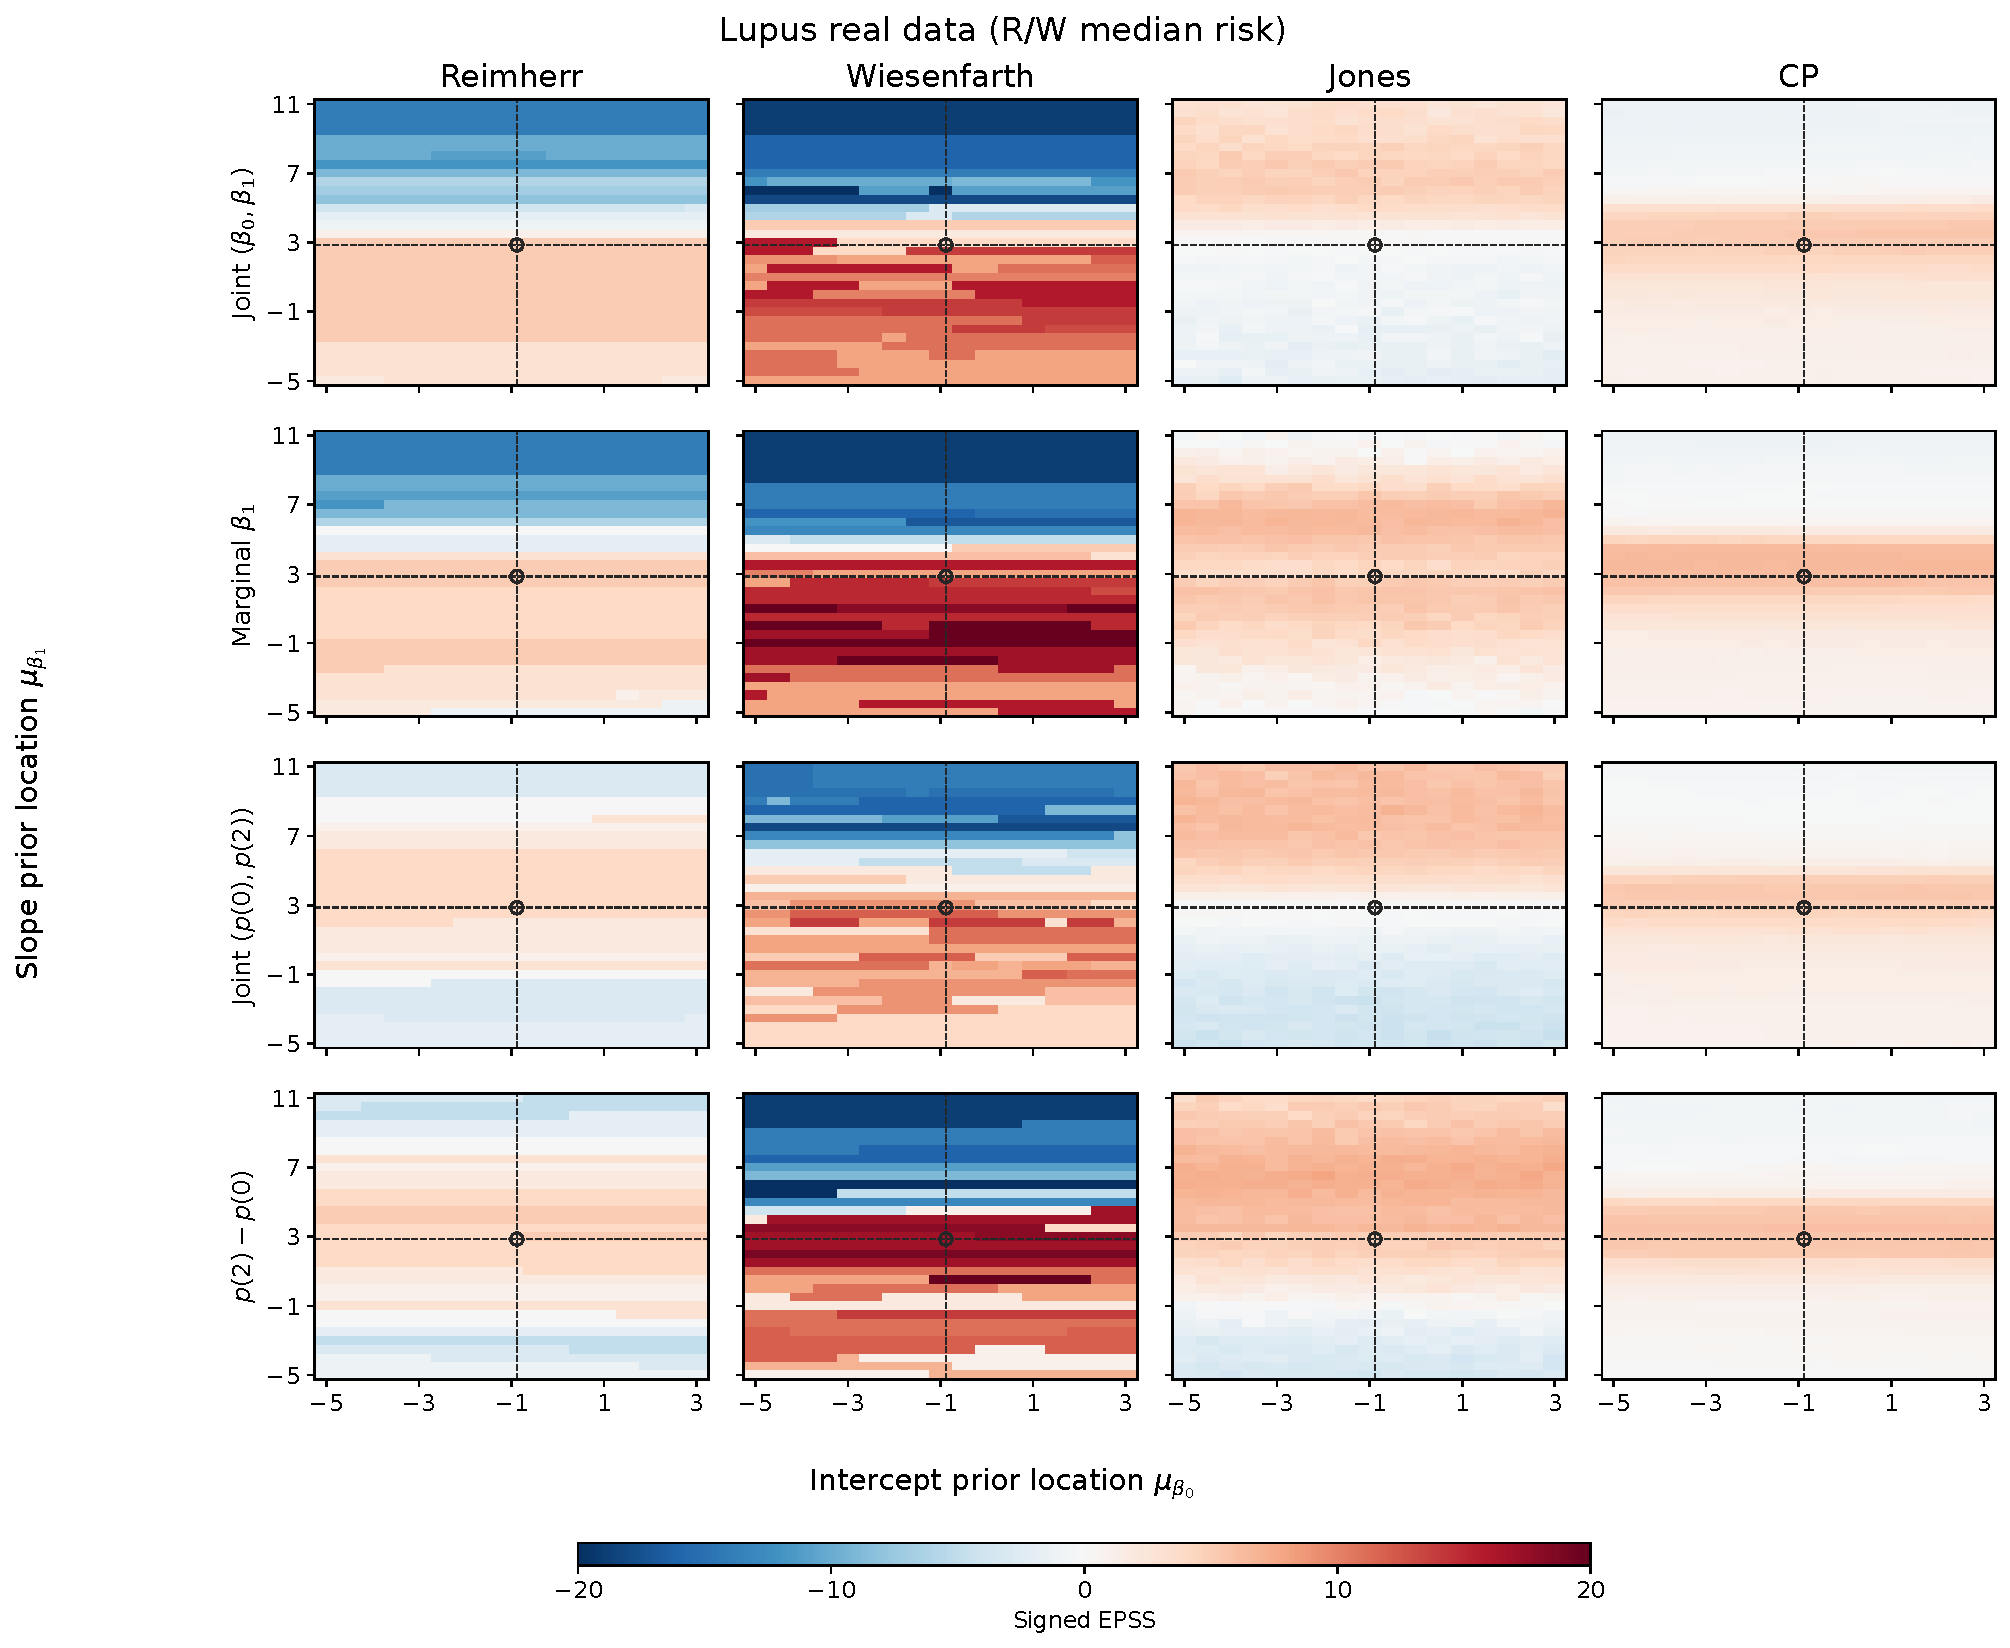
\includegraphics[width=\linewidth,height=.81\textheight,keepaspectratio]{lupus/real_4x4.pdf}
\caption{Lupus real data: four targets by four methods, with R/W median
risk. Dashed lines and the open circle mark the observed-data MLE, not a
known truth. All panels use the same 561 prior locations and EPSS scale
$[-20,20]$.}
\end{figure}
\FloatBarrier

\subsection{Simulation}
The predictor positions remain fixed. For $r=0,\ldots,29$,
\[
 Y_i^{(r)}\sim\operatorname{Bernoulli}
 \left\{\logit^{-1}(-1+3x_i^\star)\right\},\qquad
 (\beta_0^{\mathrm{true}},\beta_1^{\mathrm{true}})=(-1,3).
\]
The three displayed targets are $(\beta_0,\beta_1)$, $\beta_0$, and $\beta_1$.
All 30 datasets use the priors, grid, internal repetitions, and method
settings above. The displayed EPSS is averaged across datasets after
each dataset's median-risk or pathwise matching. Internal risk-Monte-Carlo
stability has not been certified by increasing $B$.
\begin{figure}[p]
\centering
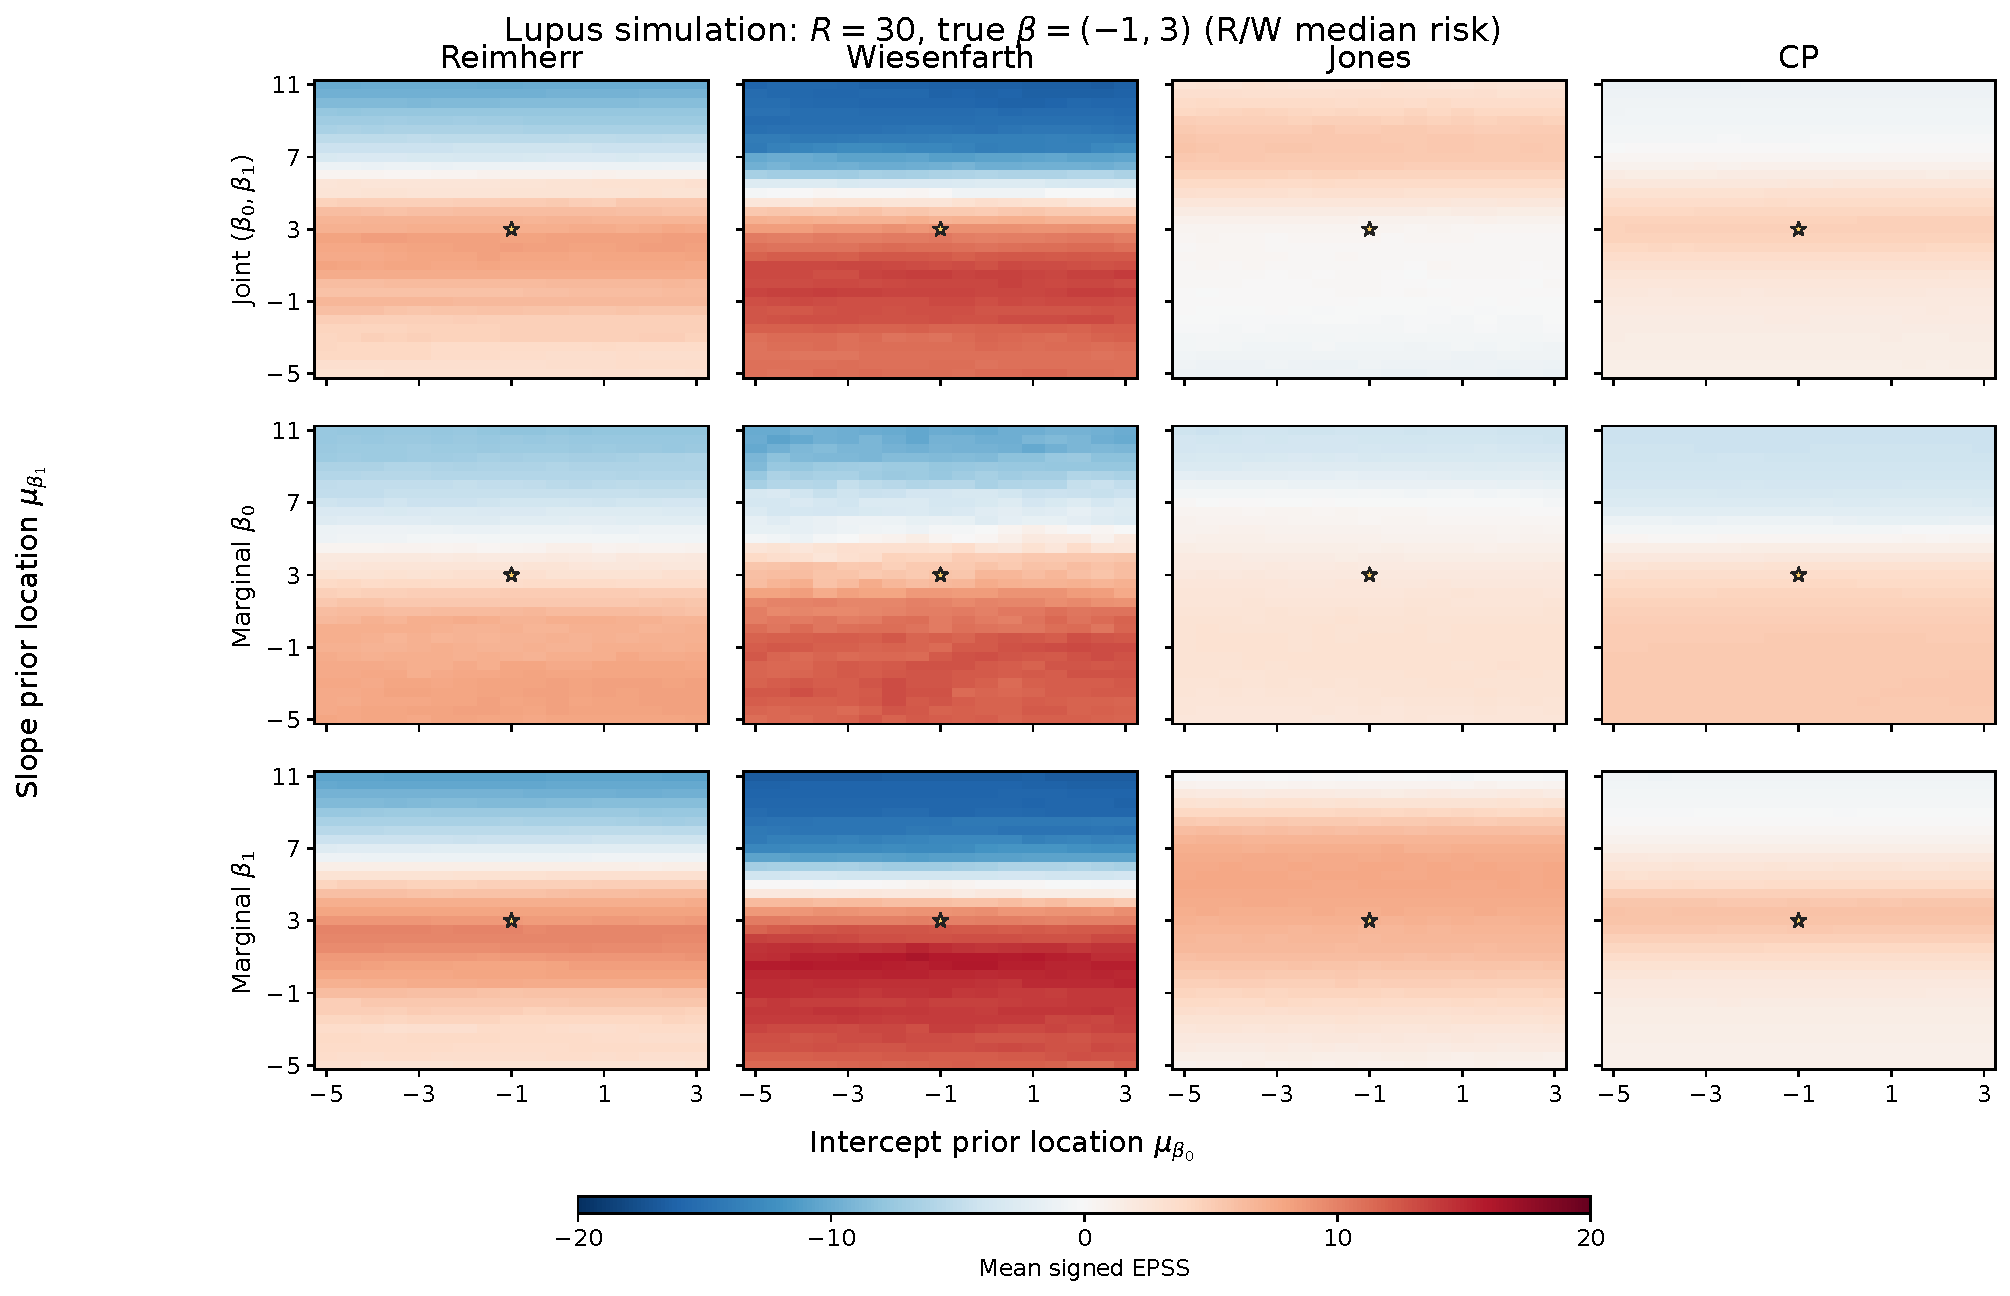
\includegraphics[width=\linewidth,height=.78\textheight,keepaspectratio]{lupus/simulation_3x4.pdf}
\caption{Lupus simulation: mean EPSS over 30 datasets, with median-risk
Reimherr and Wiesenfarth. Rows are the joint coefficient target and the
two coefficient marginals. The star marks the generating coefficients
$(-1,3)$; all panels use the common EPSS scale $[-20,20]$.}
\end{figure}
\FloatBarrier

\section{Hierarchical normal model: Eight Schools}

\subsection{Data, likelihood, and hyperpriors}
The eight estimated treatment effects and known standard errors are
\[
 y=(28,8,-3,7,-1,1,18,12),\qquad
 s=(15,10,16,11,9,11,10,18).
\]
For $j=1,\ldots,8$,
\[
 y_j\mid\theta_j\sim\Normal(\theta_j,s_j^2),\qquad
 \theta_j\mid\mu,\tau\sim\Normal(\mu,\tau^2),\qquad
 y_j\mid\mu,\tau\sim\Normal(\mu,s_j^2+\tau^2).
\]
One EPSS unit is one school summary $(y_j,s_j)$, not one pupil. The
independent hyperpriors are
\begin{align*}
 b:\quad&\mu\sim\Normal(0,25^2),&\tau&\sim\operatorname{half\text{-}t}_4(25),\\
 \pi_{\tau_0}:\quad&\mu\sim\Normal(0,25^2),&\tau&\sim\operatorname{half\text{-}t}_4(\tau_0).
\end{align*}
The 100-point prior-scale grid is
\[
 \tau_0\in\{0.25,0.50,\ldots,10\}\cup
 \{10.5,11,\ldots,30\}\cup\{31,32,\ldots,50\}.
\]
Here $\tau_0$ is a scale, not a location; all half-$t$ priors have mode zero,
and the informative prior equals the baseline at $\tau_0=25$.
The four targets, in row order, are
\[
 (\mu/10,\log(\tau/10)),\quad(\mu/10,\tau^2/100),\quad
 \log(\tau/10),\quad\tau^2/100.
\]
These are joint or marginal hyperparameter posteriors, not the
school-specific posteriors $p(\theta_j\mid y)$.

R/W use the posterior-MSE and squared posterior-mean losses specified
above. Both average $B=1000$ losses with reference
$z_b=\E_b[T(\mu,\tau)\mid y]$.
Reimherr resamples school pairs and uses $m=-6{:}20$;
Wiesenfarth generates likelihood pseudo-data at
$(\E_b[\mu\mid y],\E_b[\tau\mid y])$ and uses $m=-20{:}6$.
Jones and CP use 500 paths. Jones adds $m=0{:}20$ schools using one
informative-posterior $(\mu,\tau)$ draw per path: each new school draws
$s$ from the observed standard errors, then
$\theta\sim\Normal(\mu,\tau^2)$ and $y\sim\Normal(\theta,s^2)$.
CP uses $m=0{:}6$ deletions, retaining prefixes of an eight-pair bootstrap
sample, with 95\% central intervals or jointly calibrated central rectangles.
Posterior computation integrates over $\log\tau$ on an adaptive 801-node
grid and uses the analytic conditional Gaussian posterior of $\mu$;
no MCMC is used.

\subsection{Real data}
\begin{figure}[p]
\centering
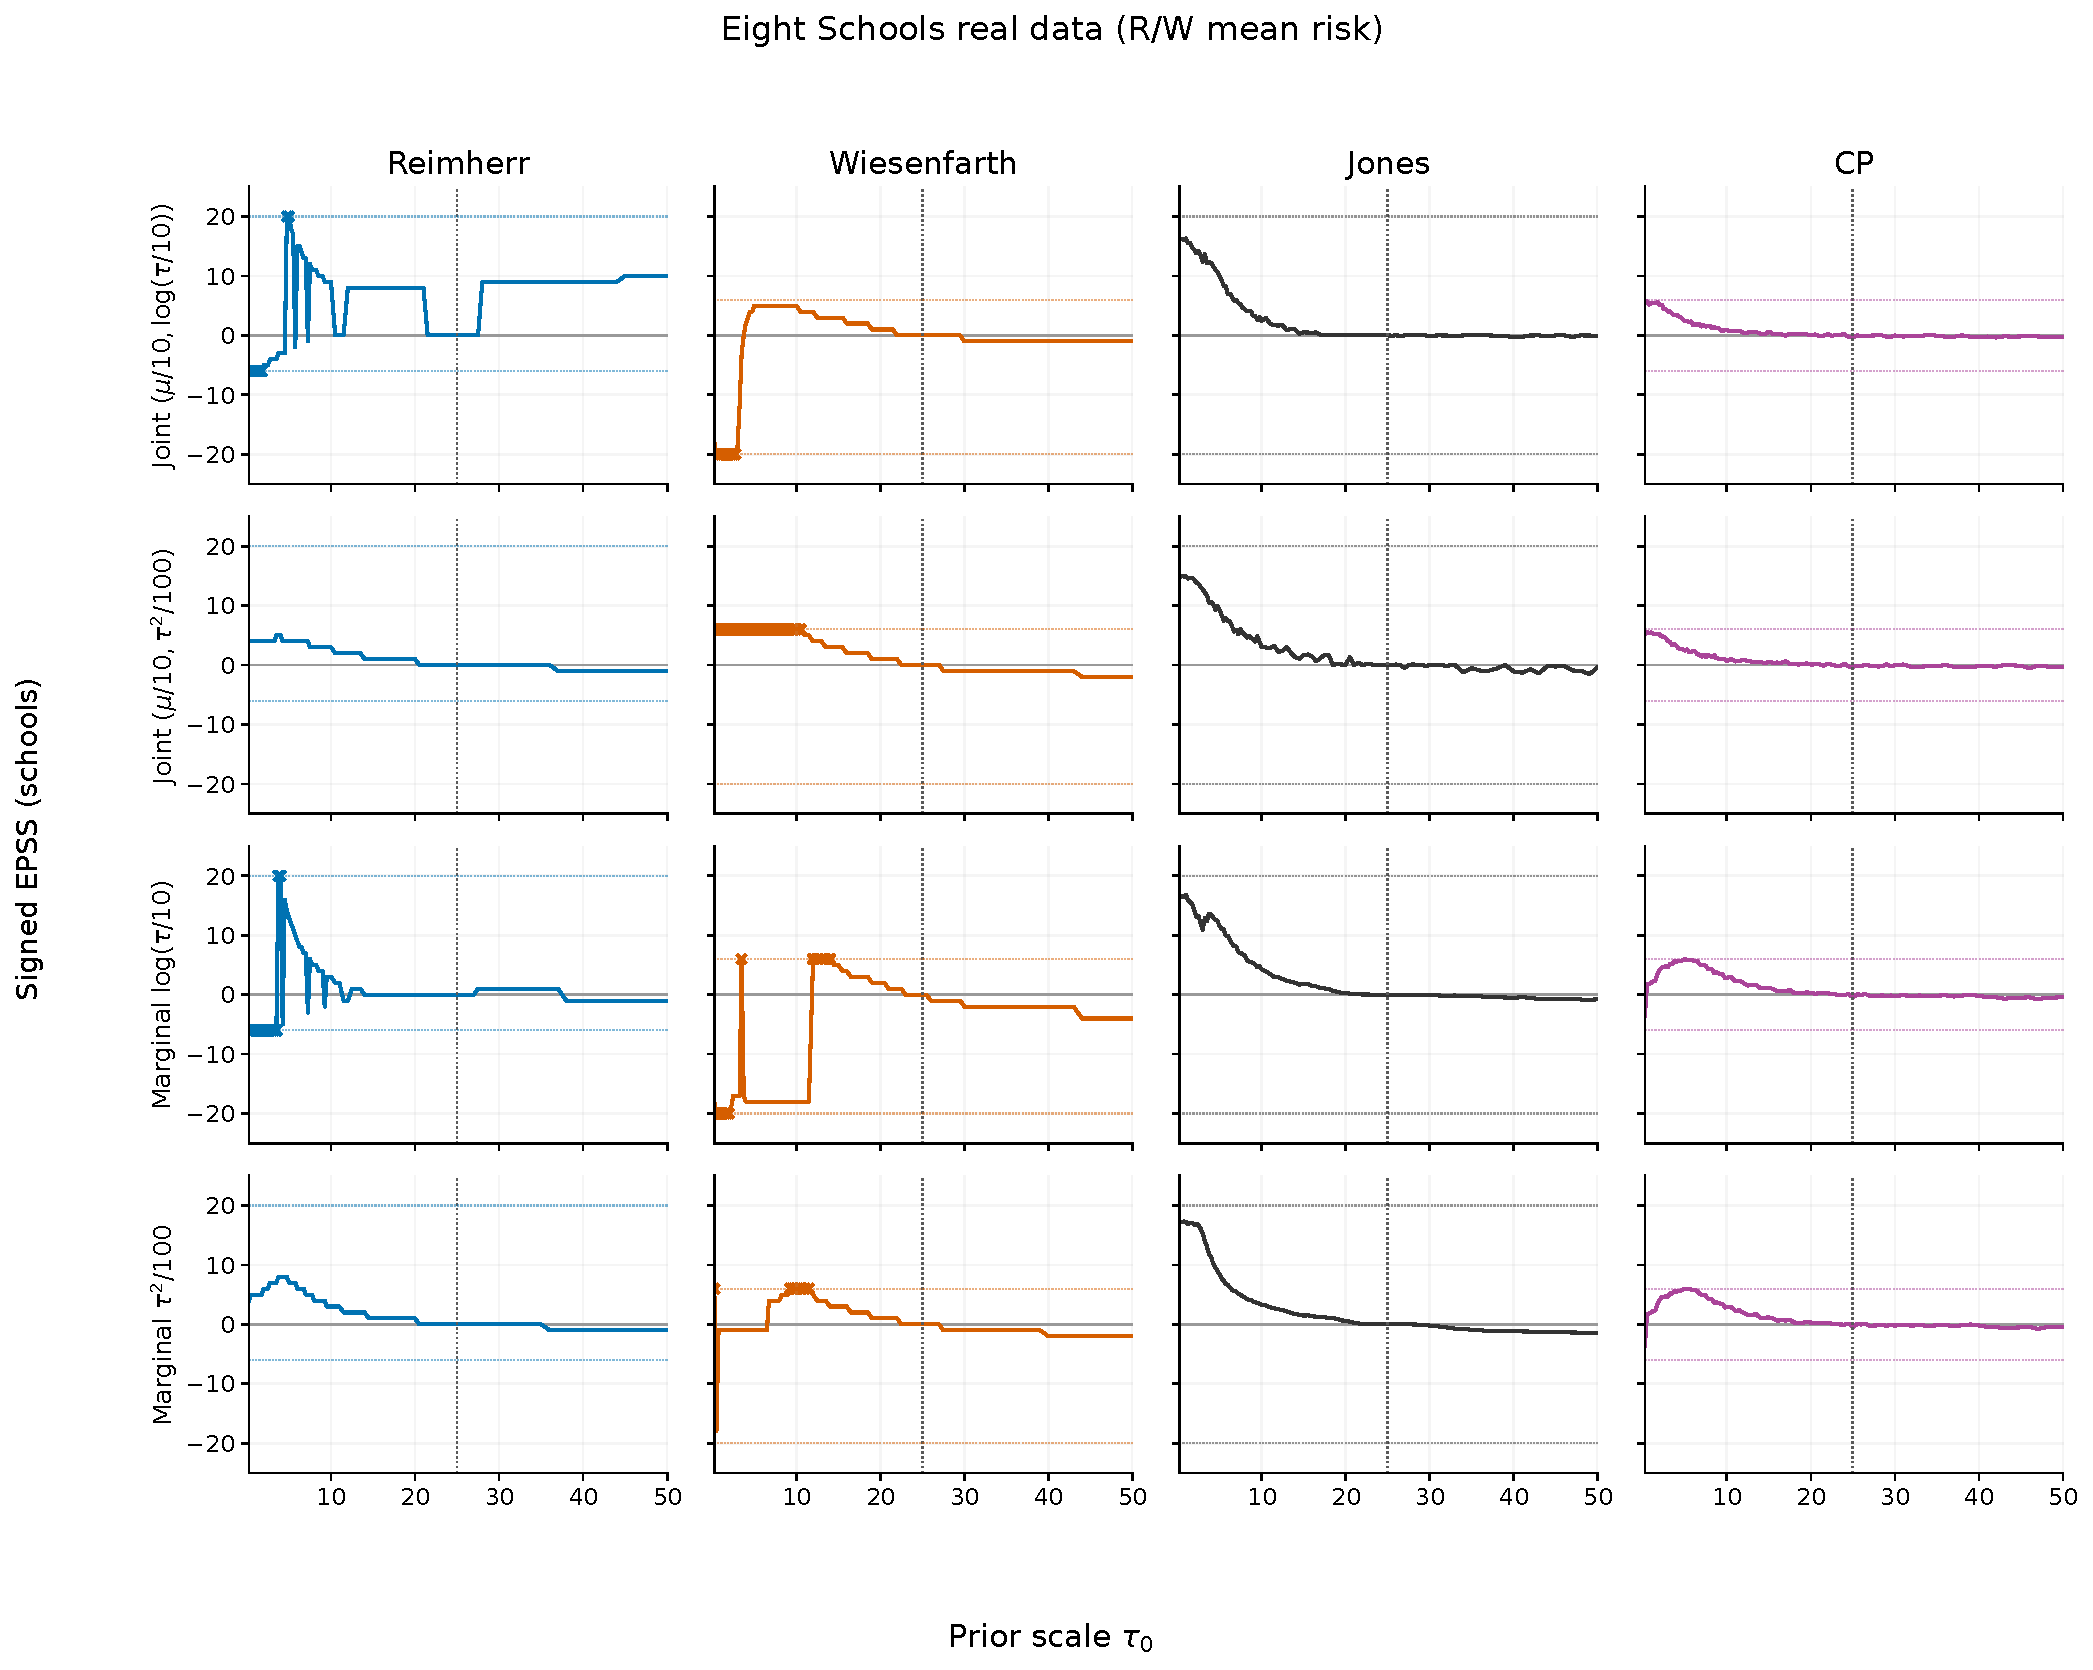
\includegraphics[width=\linewidth,height=.81\textheight,keepaspectratio]{eight_school/real_4x4.pdf}
\caption{Eight Schools real data, with R/W mean risk. The vertical dotted
line marks identical priors at $\tau_0=25$. Colored horizontal dotted
lines mark candidate limits, and crosses mark R/W endpoint selections.
There is one observed dataset and no known true hyperparameter.}
\end{figure}
\FloatBarrier

\subsection{Simulation}
For each of $R=50$ datasets, the standard errors remain fixed and
\[
 \theta_j^{(r)}\sim\Normal(8,6^2),\qquad
 y_j^{(r)}\mid\theta_j^{(r)}\sim\Normal(\theta_j^{(r)},s_j^2),
 \qquad j=1,\ldots,8.
\]
Thus $(\mu^{\mathrm{true}},\tau^{\mathrm{true}})=(8,6)$. All datasets use
the same 100 prior scales, four targets, and computational settings as
the real-data comparison.
\begin{figure}[p]
\centering
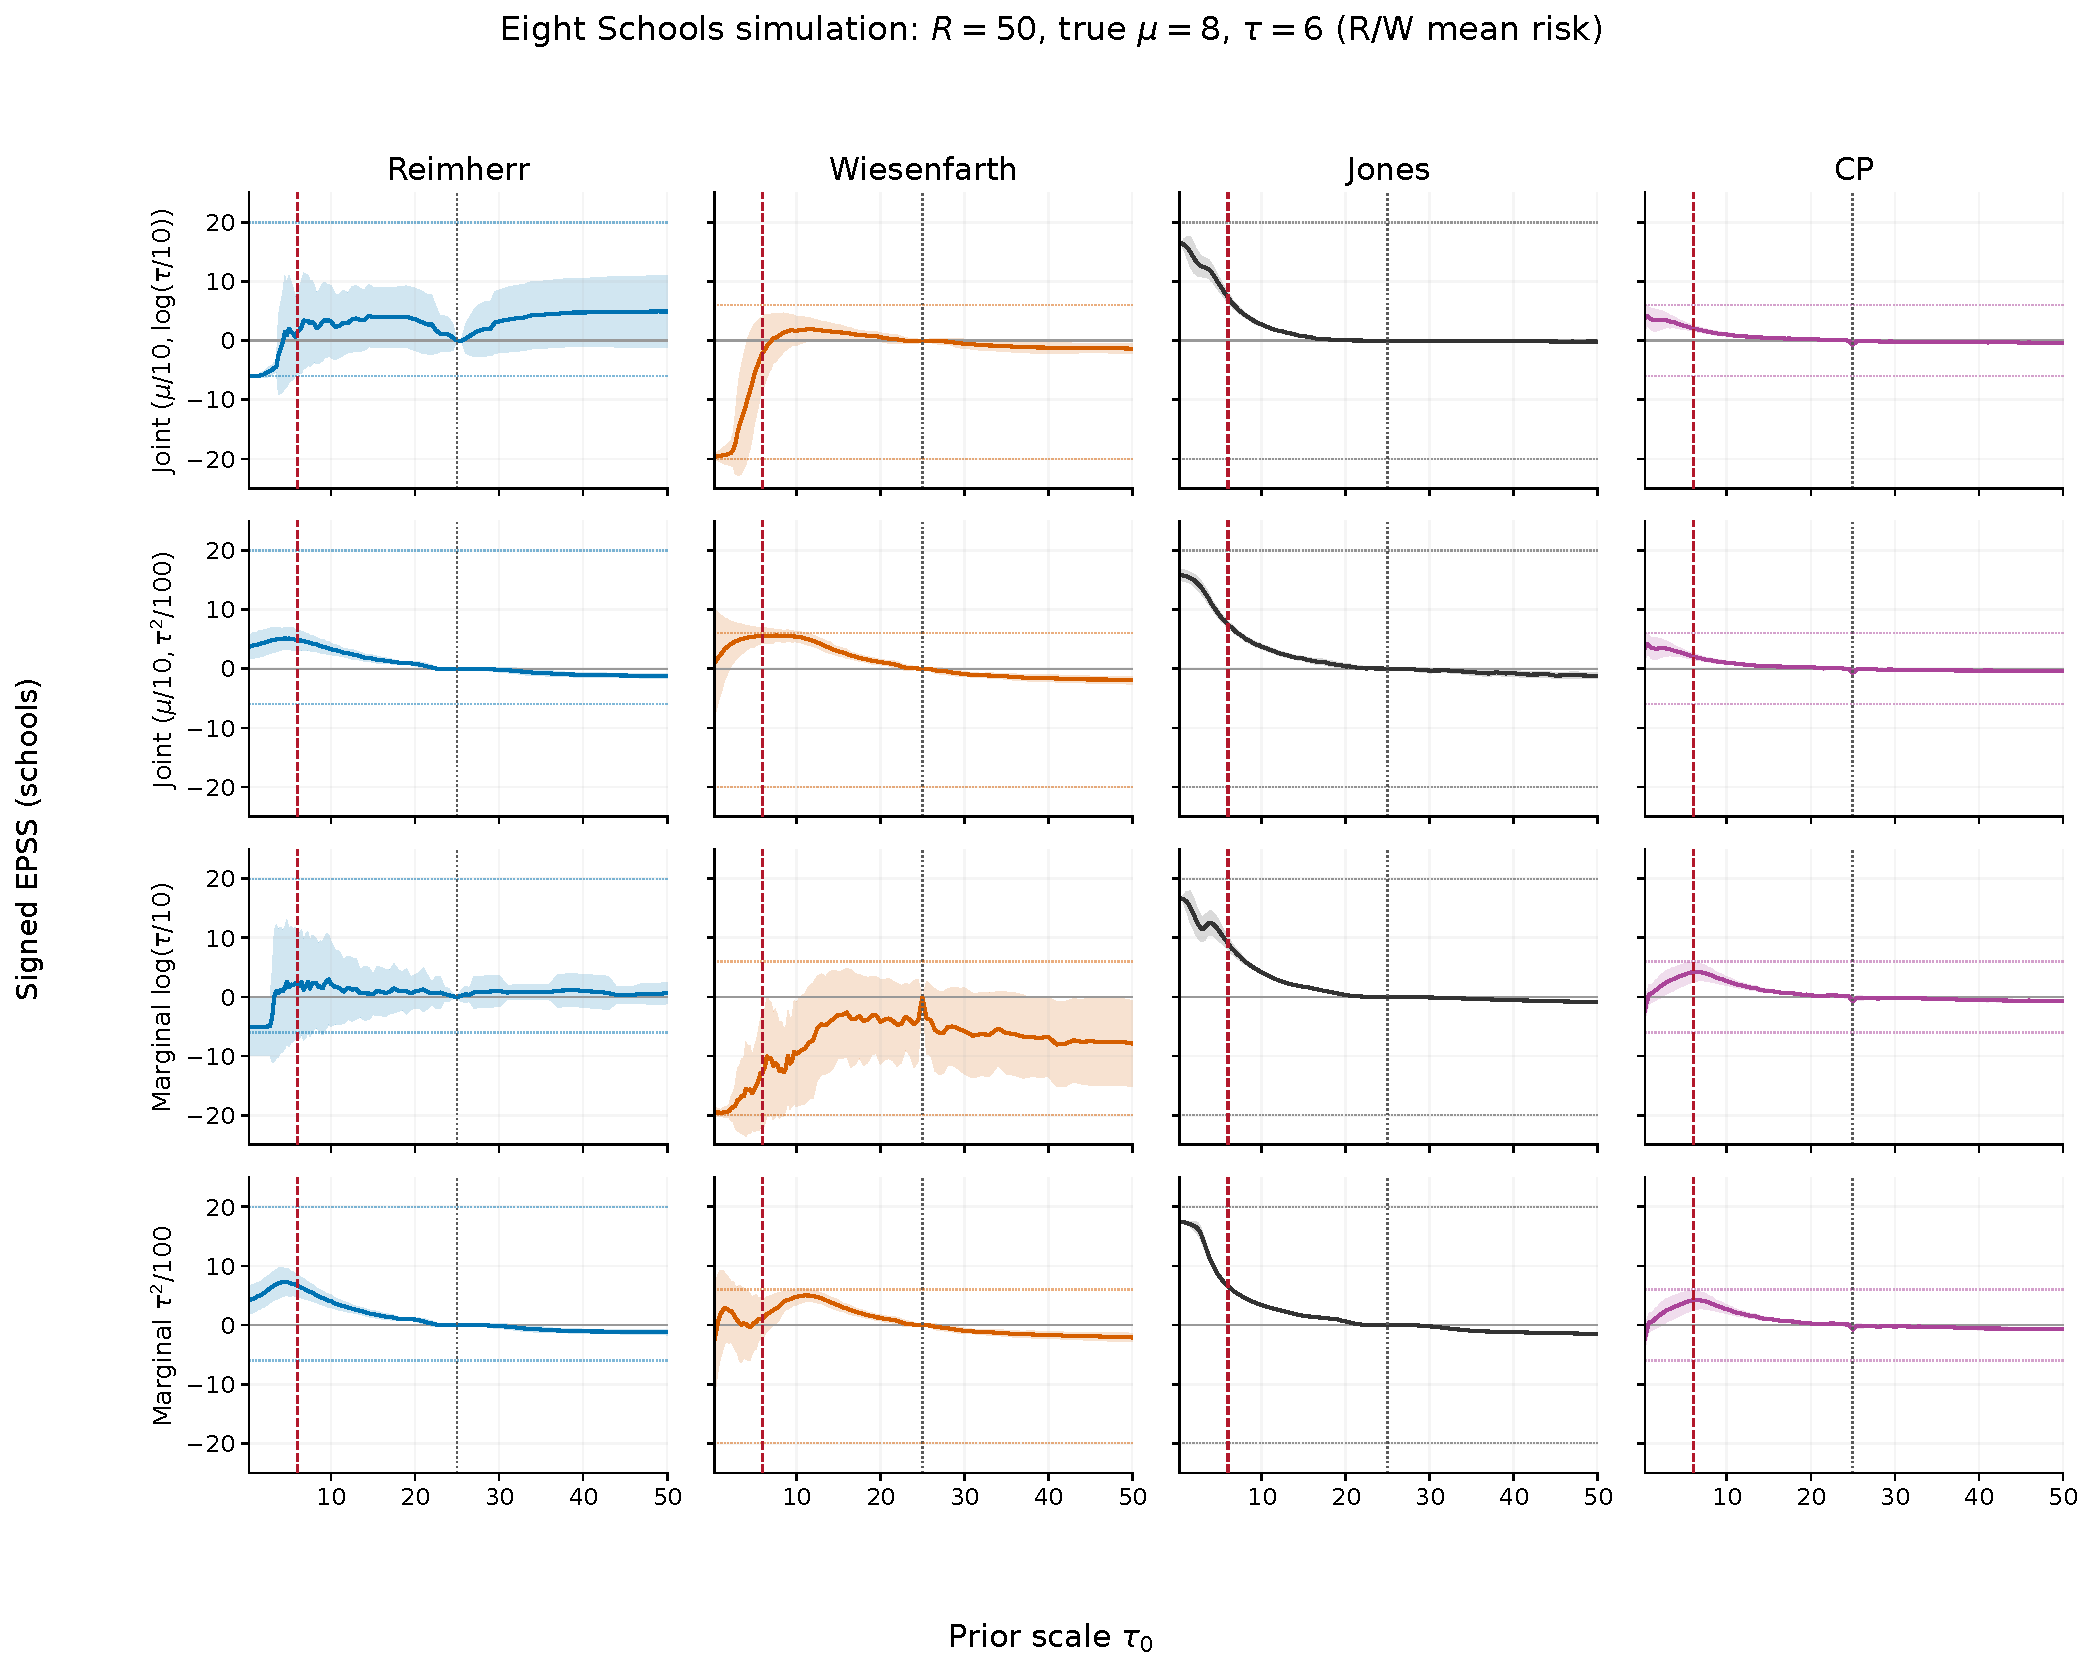
\includegraphics[width=\linewidth,height=.81\textheight,keepaspectratio]{eight_school/simulation_4x4.pdf}
\caption{Eight Schools simulation: lines are mean EPSS over 50 datasets;
bands are $\pm1$ between-dataset SD, not confidence intervals. R/W use mean
risk. Red dashed lines mark the numerical value of the generating
heterogeneity $\tau=6$ on the prior-scale axis; this does not identify
a uniquely correct prior scale. The baseline reference remains
$\tau_0=25$, and horizontal dotted lines mark candidate limits.}
\end{figure}
\end{document}
